\chapter{Realisation}
This chapter describes the implementation to extract the landmarks from biological images. This work is connected to a previous one which was implemented some operations about image segmentation by NGUYEN Hoang Thao. 
\section{Software architecture}
Extending the previous version of software, the functions of morphometry are saved in the \textbf{impls\_2015} package of the program. Besides the methods created by myself, I use some methods from the OpenCV (library for image processing) and the Qt framework (framework for C++).\\[0.2cm]
\begin{figure}[p]
    \vspace*{-3cm}
    \makebox[\linewidth]{
        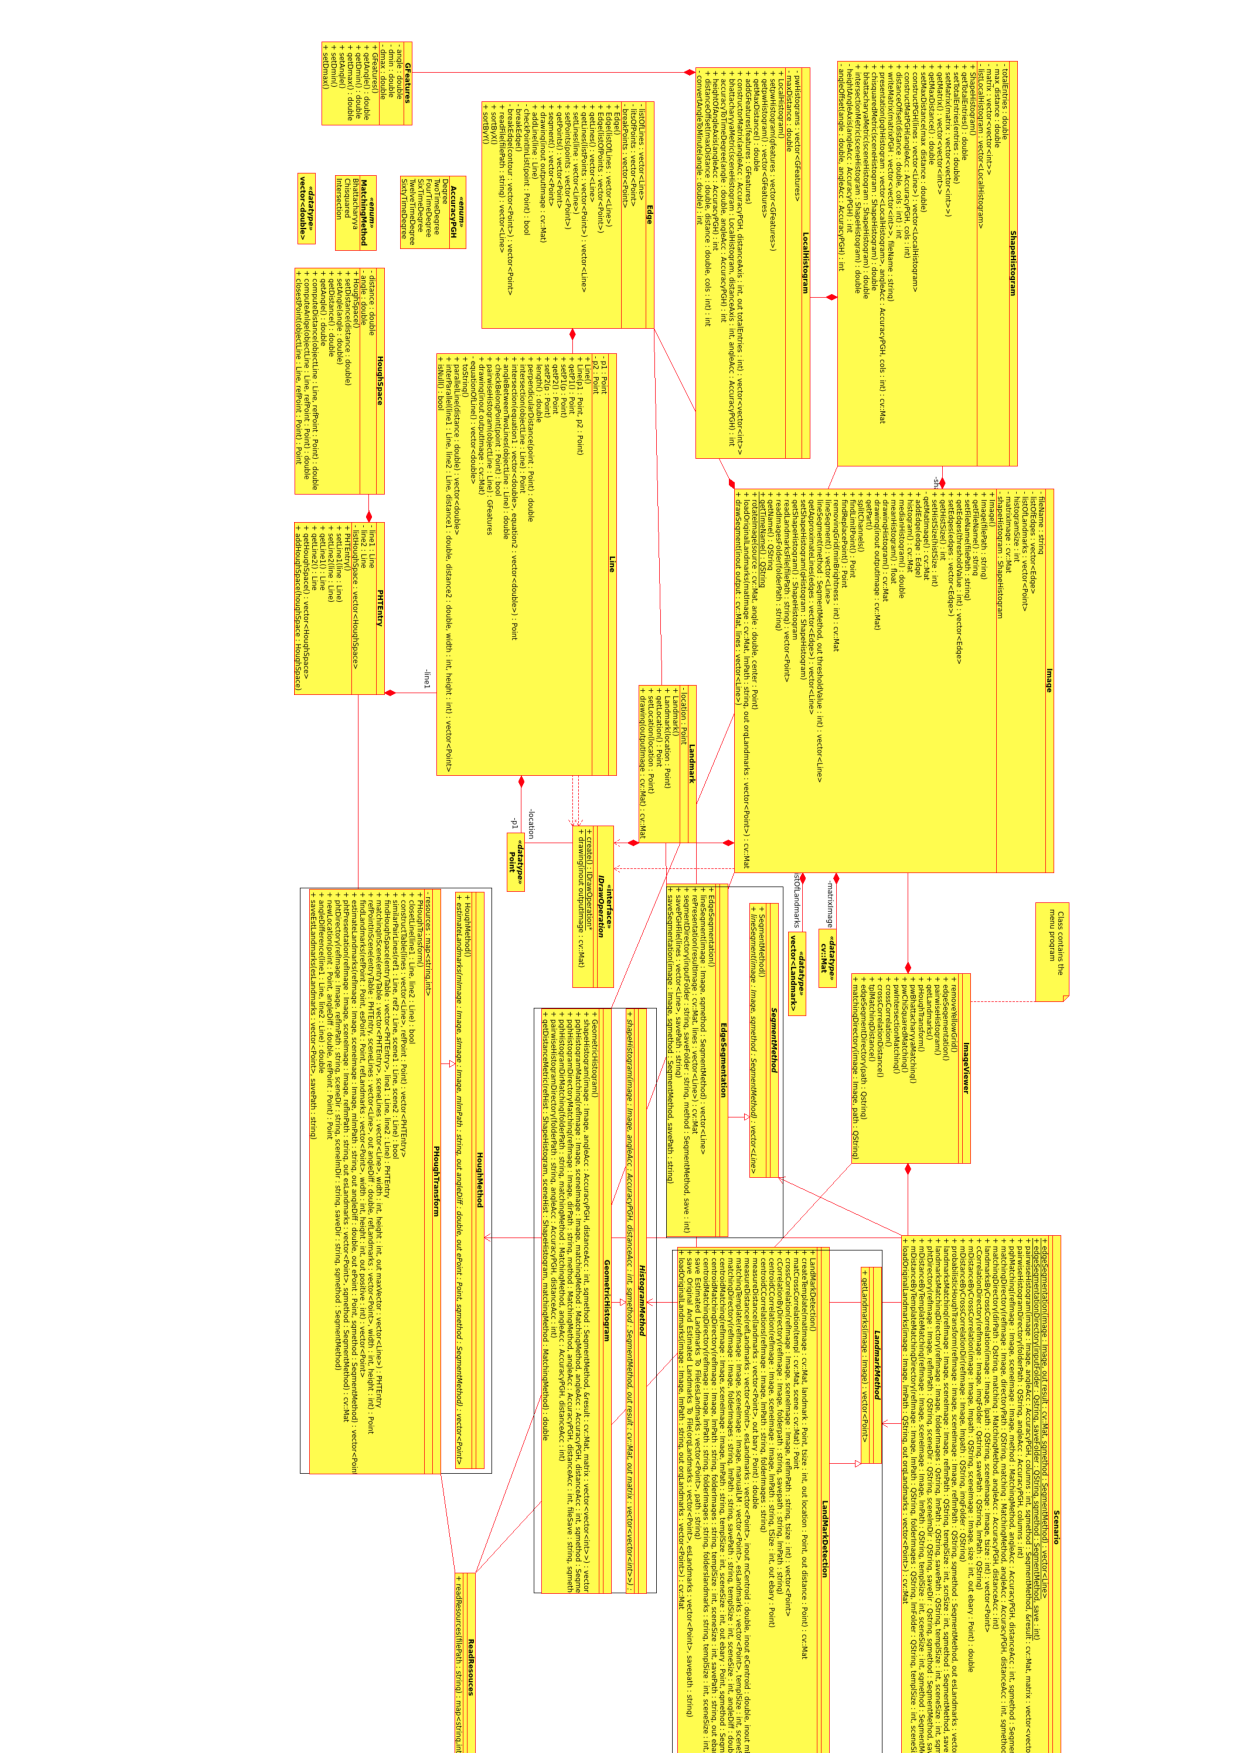
\includegraphics[width=1.1\linewidth]{images/cdiagram.pdf}
    }
    \caption{The class diagram diagram}
    \label{fig:cdiagram}
\end{figure}
The class diagram\footnote{See the full image in Appendix} in \ref{fig:cdiagram} shows main classes of my task. The \textit{mainly} methods located in the \texttt{ImageViewer} class, where contains all functions of the software. To represent the information of image and preprocessing about clear the yellow grid, we use classes such as \texttt{Line}, \texttt{Edge}, \texttt{Landmark}, \texttt{YellowGird}, \texttt{Image}. For the edge segmentation, construct the pairwise geometric histogram, probabilistic hough transform and landmarks detection, we have \texttt{GFeatures}, \texttt{LocalHistogram}, \texttt{ShapeHistogram}, \texttt{EdgeSegmentation}, \texttt{PHTransform} \texttt{LandmarkDection}. The main functions were inherated from the abstract classes \texttt{HistogramMethod}, \texttt{SegmentMethod}, \texttt{HoughMethod}, \texttt{LandmarkMethod} respective and used in \texttt{main} class (\texttt{ImageViewer}) via the \texttt{Sceneario} class. 
\section{Image preprocessing}
The \textit{Image processing} section describes information about the classes which describe the geometric objects that can be represent the image and the method to remove the yellow grid on the images.\\[0.2cm]
The \texttt{Line} class descibes the information of a straight line and its method, such as: get the length of line, compute the perpendicular distance from a point to line, find the intersection between two lines, compute the angle between two lines, find the parallel line with this line.\\[0.2cm]
The \texttt{Edge} class uses to present a curve and the methods with edge. An edge can be presented by a list of lines or a list of points. The important methods in \texttt{Edge} class are \texttt{breakEdge()} and \texttt{segment()} method. It used to break the edge into approximate lines based on the list of point constructed edge.\\[0.2cm]
The \texttt{Image} class presents the information of an image such as file name, list of edge extracted from it. Besides, \texttt{Image} class also provides the methods to get the file name of image, compute the histogram of image, remove the yellow grid (if it exist) on image, get the PGHof image, read its landmarks from a file, etc.
\section{The abstract classes}
The abstract classes contains the abstract methods get the actions on image such as segmentation, PGH construction,.... The methods are implemented by the inherit classes, respective and provide the way access to action for other classes. The abstract classes include: \texttt{HistogramMethod} class, \texttt{SegmentMethod} class, \texttt{HoughMethod} class, \texttt{LandmarkMethod} class.
\section{Edge segmentation }
\textbf{Edge segmetation} includes classes used to segment an image. Besides, the classes construct the edge which is described in previous section such as \texttt{Line, Edge,...}, we also provide the access methods for other classes.\\[0.2cm]
The \texttt{EdgeSegmentation} class provides the methods such as obtaining the lines from an image, present the result of segmentation or applying the segmentation on an image folder. The methods in \texttt{Edge segmentation} are:
\begin{itemize}
\item Extract the approximate lines of object in an image,
\item Extract the approximate lines of object in each image in a folder.
\end{itemize}
\section{Pairwise Geometric Histogram}
This section describes the classes used for PGH construction process.\\[0.2cm]
\texttt{GFeatures} class contains the relative information of the objects in PGH such as angle, minimum distance and maximum distance. It provides the methods to get and set the relative information.\\[0.2cm]
\texttt{LocalHistogram} class is constructed to contain the information when computing the PGH of a line in object. The chosen lines as reference lines, the local histogram is constructed based on recording the relating between reference line and other lines in object. Besides, it has the methods for the user to change the accuracy, such as the angle accuracy or the distance accuracy.\\[0.2cm]
\texttt{ShapeHistogram} class constructs the PGH for an object. It is constructed by on combing all PGH of the lines in an object. It also provides the methods to compute the measured distance between the pairwise geometric histograms by a matching method. The methods in this class includes:
\begin{itemize}
\item Construct the PGH for an image,
\item Construct the matrix to save the PGH result,
\item Compute the measured distance between the two PGHs based on \textit{Bhattacharyya}, \textit{Chi-Squared} or \textit{Intersection} metric.
\end{itemize}
\texttt{GeometricHistogram} class provides the access ways for other classes. By usign this class, user can compute the pairwise geometric histogram of an image and calculate the distance between the pairwise geometric histograms.
\section{Estimate the global pose (Probabilistic Hough Transform)}
This section describes the classes use probabilistic hough transform to estimate the model image from a scene image. In particular, it is estimating the reference landmarks on the scene image.\\[0.2cm]
\texttt{HoughSpace} class contains the information about the angle and distance from a line to a reference point. These information is recorded to construct the accumulator when we apply the Probabilistic Hough Transform.\\[0.2cm]
\texttt{PHTEntry} class presents each entry when constructing the reference table in the training process. Each entry contains the pair of lines and its information about angle and distance to a reference point.\\[0.2cm]
\texttt{PHoughTransform} class describes the main process when we apply the probabilistic hough transform to estimate the landmarks. It includes the methods to construct the reference table, find the reference point in scene image and estimate the landmarks. Besides, it also provides the methods to estimated the landmarks of an image on the directory of images.
\section{Refine the landmarks}
\texttt{LandmarkDetection} class provides the methods to refine the landmarks. It uses cross-correlation technique to refine the estimated landmarks. Besides, we might compute the centroid point of an object.